%\VignetteIndexEntry{FunciSNP Vignette}
%\VignetteDepends{FunciSNP}
%\VignetteKeywords{SNP}
%\VignetteKeywords{Functional}
%\VignetteKeywords{GWAS}
%\VignettePackage{FunciSNP}
%%%%%%%%%%%%%%%%%%%%%%%%%%%%%%%%%%%%%%%%%%%%%%
\documentclass[12pt,fullpage]{article}
\usepackage{amsmath,epsfig,fullpage}
\usepackage{hyperref}
\usepackage{url}
\usepackage[authoryear,round]{natbib}
%\usepackage[OT1]{fonitenc}
\usepackage{Sweave}
\usepackage{textcomp}
%%%%%%%%%%%%%%%%%%%%%%%%%%%%%%%%%%%%%%%%%%%%%%
\newcommand{\Rfunction}[1]{{\texttt{#1}}}
\newcommand{\Robject}[1]{{\texttt{#1}}}
\newcommand{\Rpackage}[1]{{\textit{#1}}}
\newcommand{\Rclass}[1]{{\textit{#1}}}
\newcommand{\Rmethod}[1]{{\textit{#1}}}
%%%%%%%%%%%%%%%%%%%%%%%%%%%%%%%%%%%%%%%%%%%%%%
\author{Simon G. Coetzee$^\ddagger$\footnote{scoetzee NEAR gmail POINT com},
    Suhn K. Rhie$^\ddagger$, Benjamin P. Berman$^\ddagger$,\\Gerhard A.
        Coetzee$^\ddagger$ and Houtan Noushmehr$^\ddagger$\footnote{houtana NEAR
            gmail POINT com}}
%%%%%%%%%%%%%%%%%%%%%%%%%%%%%%%%%%%%%%%%%%%%%%
\begin{document}
\title{Using the FunciSNP package\\`FunciSNP: An R/Bioconductor Tool \\
Integrating Functional Non-coding Datasets with Genetic Association Studies to\\
 Identify Candidate Regulatory SNPs'}
\maketitle
%%% Affiliation %%%
\begin{center}
$^\ddagger$Norris Cancer Center\\Keck School of Medicine\\University of Southern
California\\Los Angeles, CA, USA
\end{center}
%%%%%%%%%%%%%%%%%%%%%%%%%%%%%%%%%%%%%%%%%%%%%%
\tableofcontents
%%%%%%%%%%%%%%%%%%%%%%%%%%%%%%%%%%%%%%%%%%%%%%
%%%%%%%%%%%%%%%%%%%%%%%%%%%%%%%%%%%%%%%%%%%%%%
\section{Introduction}
%%%%%%%%%%%%%%%%%%%%%%%%%%%%%%%%%%%%%%%%%%%%%%
%%%%%%%%%%%%%%%%%%%%%%%%%%%%%%%%%%%%%%%%%%%%%%

\Rpackage{FunciSNP} assist in identifying putative functional SNP in LD to
previously annotated GWAS SNPs (tagSNP). Extracting information from the 1000
genomes database (1kg) by relative genomic position of GWAS tagSNP currated
for a particular trait or disease, FunciSNP aims to integrate the two
information with sequence information provided by peaks identified from
high-throughput sequencing. FunciSNP assumes user will provide peaks identified
using any available ChIP peak algorithm, such as FindPeaks, HOMER, or SICER.
\Rpackage{FunciSNP} will currate all 1kg SNPs which are in linkage
disequilibrium (LD) to a known disease associated tagSNP and more importantly
determine if the 1kg SNP in LD to the tagSNP overlaps a genomic biological
feature.

Correlated SNPs are
directly imported from the current public release of the 1000 genomes database.
1000 genomes ftp servers available for the 1000 genomes public data: 

\begin{itemize}
\item National Center for Biotechnology Information
(NCBI)\footnote{\url{ftp://ftp-trace.ncbi.nih.gov/1000genomes/}}
\item European Bioinformatics Institute
(EBI)\footnote{\url{ftp://ftp.1000genomes.ebi.ac.uk/vol1/}}
\end{itemize}

Correlated SNPs in LD to a tagSNP and overlapping genomic biological features
are known as putative functional SNPs.

This vignette provides a `HOW-TO' guide in setting up and running
\Rpackage{FunciSNP} on your machine. FunciSNP was developed with the idea that a
user will have uninterupted high-speed internet access as well as a desktop
machine with  more than 4 multiple cores. If user is using a windows machine,
multiple cores options will not work and thus total time to complete
initial FunciSNP analysis will take longer than expected. Be sure you
have uninterupted computing power when using a windows machine. If using
a linux machine, please use `screen' (see `man screen' for more
information).

\subsection{Benchmark}
Using a 64bit Linux machine running 11.04 Ubuntu OS with 24G RAM and 8 cores
connected to a academic high-speed internet port, the amount of time to complete
99 tagSNP across 20 different biofeatures took less than 30 min to complete. We
anticipate about 2 hours to complete the same analysis using one core.

\subsection{Genome-Wide Association Studies SNP (GWAS SNP)}
Genome-wide association studies (GWASs) have yielded numerous single nucleotide
polymorphisms (SNPs) associated with many phenotypes. In some cases tens of
SNPs, called tagSNPs, mark many loci of single complex diseases such as prostate
(> 50 loci), breast (> 20 loci), ovarian (>10 loci), colorectal (>20 loci) and
brain cancer (>5 loci) for which functionality remains unknown. Since most of
the tagSNPs (>80\%) are found in non-protein coding regions, finding direct
information on the functional and/or causal variant has been an important
limitation of GWAS data interpretation.

\subsection{1000 genomes project (1kg)}
The 1000 genomes project recently released a catalog of most human genomic
variants (minor allele frequency of >0.1\%) across many different ethnic
populations. Initially, the 1000 genomes project goal was to sequence up to 1000
individuals, but has since sequenced more than 2000 individuals, thereby
increasing our current knowledge of known genomic variations which currently
sits at just over 50 million SNPs genome wide (approx. 2\% of the entire genome
        and on average 1 SNP every 60 base pairs)

\subsection{Genomic features (Biofeatures)}
With the advent of advanced sequencing technologies (next-generation sequencing,
        NGS), genomic regulatory areas in non-coding regions have been well
characterized and annotated. Coupled with chromatin immuno-precipitation for a
protein (e.g. transcription factor of histone) of interest, also known as
ChIPseq, the technology have provided us with a unique view of the genomic
landscape, thereby providing a wealth of new knowledge for genomics
research. Work by large consortia groups such as the Encyclopedia of DNA Elements
(ENCODE), the Roadmap Epigenomics Mapping Consortium and The Cancer
Genome Atlas (TCGA), have made publicly available a growing catalog of many
different histone marks, transcription factors and genome-wide sequencing
datasets for a variety of different diseases and cell lines, including well
characterized cancer cell lines such as MCF7 (breast cancer), HCT116 (colon
        cancer), U87 (brain cancer) and LNCaP (prostate cancer). 

%%%%%%%%%%%%%%%%%%%%%%%%%%%%%%%%%%%%%%%%%%%%%%
%%%%%%%%%%%%%%%%%%%%%%%%%%%%%%%%%%%%%%%%%%%%%%
\section{Installing and Loading FunciSNP}
%%%%%%%%%%%%%%%%%%%%%%%%%%%%%%%%%%%%%%%%%%%%%%
%%%%%%%%%%%%%%%%%%%%%%%%%%%%%%%%%%%%%%%%%%%%%%

Currently, there are two options to obtain a copy of \Rpackage{FunciSNP}: 

\begin{itemize}
\item Download current source code from Coetzee's
lab\footnote{\url{http://coetzeeseq.usc.edu/publication/Coetzee_SG_et_al_2012/}}
\item Download and install from
Bioconductor\footnote{\url{http://www.bioconductor.org}}
\end{itemize}

If you download the source code from either method above, you can install
\Rpackage{FunciSNP} by following the instructions described in R CRAN. By
installing \Rpackage{FunciSNP} from source, the package assumes you have all the
required libraries installed.

\begin{itemize}
\item Rsamtools (>= 1.6.1)
\item rtracklayer(>= 1.14.1)
\item GGtools (>= 4.0.0)
\item methods
\item ChIPpeakAnno (>= 2.2.0)
\item GenomicRanges
\item TxDb.Hsapiens.UCSC.hg19.knownGene
\item VariantAnnotation
\item plyr
\item org.Hs.eg.db
\item snpStats
\end{itemize}

The following loads the \Rpackage{FunciSNP} library in R.

\begin{Schunk}
\begin{Sinput}
> options(width=80);
> library(FunciSNP);
> package.version("FunciSNP");
\end{Sinput}
\begin{Soutput}
[1] "0.1.14"
\end{Soutput}
\end{Schunk}

%%%%%%%%%%%%%%%%%%%%%%%%%%%%%%%%%%%%%%%%%%%%%%
%%%%%%%%%%%%%%%%%%%%%%%%%%%%%%%%%%%%%%%%%%%%%%
\section{Running getFSNPs to identify putative functional SNPs}
%%%%%%%%%%%%%%%%%%%%%%%%%%%%%%%%%%%%%%%%%%%%%%
%%%%%%%%%%%%%%%%%%%%%%%%%%%%%%%%%%%%%%%%%%%%%%

Before running \Rmethod{getFSNPs}, two input files are required. A list of
tagSNPs and a folder with all available biological features (peak files in BED
        format).

\subsection{Create a GWAS SNP file}

GWAS SNPs (tagSNP) should be listed in a tab or whitespace separated file. Three
columns are required for each tagSNP: 

\begin{itemize}
\item Position (chrom:position)
\item rsID (rsXXXXXXXX)
\item population (EUR, AFR, AMR, ASN, or ALL)
\end{itemize}

`Positon' should be the exact postion for each rsID as reported by human genome
build hg19 (chrom:postion). `rsID' should contain a unique rsID as determined by
the 1000 genomes database (1kg)\footnote{Be sure the rsID is located in this
browser: \url{http://browser.1000genomes.org/}} for each identified `tagSNP'.
Population should be a three letter code to determine original ethnic population
for which the associated `tagSNP' was identified. The three letter code should
be either European (EUR), Asian (ASN), African (AFR), American (AMR), or All
(ALL). List each tagSNP per ethnic population. If similar rsID was identified in
multiple ethnic population, list each duplicate tagSNP separately with the
appropriate ethnic pouplation.

Several GWAS SNPs significantly associated with Glioblastoma multiforme
(GBM)\footnote{See \url{http://www.snpedia.com/index.php/Glioma}} were collected
for this example. GBM is a brain cancer with median survival at less than 12
months, making this form of cancer one of the most aggressive of all cancer
types. Currently, there is no known function of any of these associated tagSNPs.
In this example, GBM includes lower grade glioma, therefore we use the `glioma'
to label all objects.

\begin{Schunk}
\begin{Sinput}
> ## Full path to the example GWAS SNP regions file for Glioblastoma 
> #  (collected from SNPedia on Jan 2012)
> glioma.snp <- file.path(system.file('extdata', package='FunciSNP'), 
+ dir(system.file('extdata',package='FunciSNP'), pattern='.snp$'));
> gsnp <- read.delim(file=glioma.snp,sep=" ",header=FALSE);
> gsnp;
\end{Sinput}
\begin{Soutput}
            V1        V2  V3
1 11:118477367  rs498872 EUR
2    5:1286516 rs2736100 ASN
3   9:22068652 rs4977756 EUR
4  20:62309839 rs6010620 EUR
\end{Soutput}
\end{Schunk}

Now, \Robject{glioma.snp} contains the full path to the GWAS tagSNP. 

\subsection{Biofeatures in BED format}

Each biofeature used to identify correlated SNP should be in standard BED
format\footnote{See UCSC FAQ: \url{http://genome.ucsc.edu/FAQ/FAQformat}}. Each
biofeature should be stored in one folder and should have file extension
`*.bed'.

Here is an example of three different biofeatures used for this glioma example.
NRSF and PolII (both transcription factors) where extracted from a recent
release of ENCODE, as well as promoters of approximately 38,000 gene
transcription start sites (TSS). Promoters are identified as +1000 to -100 base
pair of each annotated TSS. In addition, we include all known DNAseI sites as supplied by ENCODE as well as FAIRE data. In additoin, we used known CTCF sites to differentiate the DNAseI. The DNAseI and FAIRE data were extracted in April of 2012 and they represent the best known regions across several different cell lines. In addition, for the FAIRE data, we selected peaks with p-values less than 0.01.

\begin{Schunk}
\begin{Sinput}
> ## Full path to the example biological features BED files 
> #  derived from the ENCODE project for Glioblastoma U-87 cell lines.
> glioma.bio <- system.file('extdata',package='FunciSNP');
> #user supplied biofeatures
> as.matrix(list.files(glioma.bio, pattern='.bed$'));
\end{Sinput}
\begin{Soutput}
     [,1]               
[1,] "TFBS_Nrsf_U87.bed"
[2,] "TFBS_Pol2_U87.bed"
\end{Soutput}
\begin{Sinput}
> #FunciSNP builtin biofeatures
> as.matrix(list.files(paste(glioma.bio, "/builtInFeatures", sep=""),
+             pattern='.bed$'));
\end{Sinput}
\begin{Soutput}
     [,1]                             
[1,] "CTCF_only.known.bed"            
[2,] "EncodeDnaseI_only.known.bed"    
[3,] "EncodeDnaseI_withCTCF.known.bed"
[4,] "EncodeFaire.known.bed"          
[5,] "knownGene.Promoters.known.bed"  
\end{Soutput}
\begin{Sinput}
> nrsf.filename <- list.files(glioma.bio, pattern='.bed$')[1];
> pol2.filename <- list.files(glioma.bio, pattern='.bed$')[2];
> ctcf.filename <- list.files(paste(glioma.bio, "/builtInFeatures", sep=""),
+         pattern='.bed$')[1];
> dnase1.filename <- list.files(paste(glioma.bio, "/builtInFeatures", sep=""),
+         pattern='.bed$')[2];
> dnase1ctcf.filename <- list.files(paste(glioma.bio, "/builtInFeatures", sep=""),
+         pattern='.bed$')[3];
> faire.filename <- list.files(paste(glioma.bio, "/builtInFeatures", sep=""),
+         pattern='.bed$')[4];
> prom.filename <- list.files(paste(glioma.bio, "/builtInFeatures", sep=""),
+         pattern='.bed$')[5];
> Nrsf <- read.delim(file=paste(glioma.bio, nrsf.filename,sep="/"), sep="\t",
+ header=FALSE);
> PolII <- read.delim(file=paste(glioma.bio, pol2.filename,sep="/"), sep="\t",
+ header=FALSE);
> Ctcf <- read.delim(file=paste(glioma.bio, "builtInFeatures", ctcf.filename,sep="/"), sep="\t",
+ header=FALSE);
> Dnase1 <- read.delim(file=paste(glioma.bio, "builtInFeatures", dnase1.filename,sep="/"), sep="\t",
+ header=FALSE);
> Dnase1Ctcf <- read.delim(file=paste(glioma.bio, "builtInFeatures", dnase1ctcf.filename,sep="/"), sep="\t",
+ header=FALSE);
> Faire <- read.delim(file=paste(glioma.bio, "builtInFeatures", faire.filename,sep="/"), sep="\t",
+ header=FALSE);
> Promoters <- read.delim(file=paste(glioma.bio, "builtInFeatures", prom.filename,sep="/"), sep="\t",
+ header=FALSE);
> dim(Nrsf);
\end{Sinput}
\begin{Soutput}
[1] 1264    6
\end{Soutput}
\begin{Sinput}
> dim(PolII);
\end{Sinput}
\begin{Soutput}
[1] 10918     6
\end{Soutput}
\begin{Sinput}
> dim(Ctcf);
\end{Sinput}
\begin{Soutput}
[1] 9917    3
\end{Soutput}
\begin{Sinput}
> dim(Dnase1);
\end{Sinput}
\begin{Soutput}
[1] 175508      3
\end{Soutput}
\begin{Sinput}
> dim(Dnase1Ctcf);
\end{Sinput}
\begin{Soutput}
[1] 4978    3
\end{Soutput}
\begin{Sinput}
> dim(Faire);
\end{Sinput}
\begin{Soutput}
[1] 211650      3
\end{Soutput}
\begin{Sinput}
> dim(Promoters);
\end{Sinput}
\begin{Soutput}
[1] 39701     6
\end{Soutput}
\begin{Sinput}
> ## Example of what the BED format looks like:
> head(Nrsf);
\end{Sinput}
\begin{Soutput}
    V1        V2        V3                      V4 V5 V6
1 chr5 178601706 178602140 Merged-chr5-178601923-1  0  +
2 chr5 178850156 178850592 Merged-chr5-178850374-1  0  +
3 chr5 179015119 179015553 Merged-chr5-179015336-1  0  +
4 chr7     23844     24636     Merged-chr7-24240-1  0  +
5 chr7     65601     66065     Merged-chr7-65833-1  0  +
6 chr7    128907    129421    Merged-chr7-129164-1  0  +
\end{Soutput}
\end{Schunk}

As an example, \Robject{Nrsf} was created to illustrate the format needed for
each biofeatures. To run getFSNPs, only the path to the folder to each
biofeature is required (\Robject{glioma.bio}).

\subsection{getFSNPs analysis using two inputs}

To run the example data could take more than 5 minutes, thus the R code is
commented out for this tutorial. If you are interested in running the glioma
example from scratch, please uncomment the following and rerun in your R
session. NOTE: The main method to run FunciSNP is \Rmethod{getFSNPs}.

\begin{Schunk}
\begin{Sinput}
> ## FunciSNP analysis, extracts correlated SNPs from the 
> ## 1000 genomes db ("ncbi" or "ebi") and finds overlaps between 
> ## correlated SNP and biological features and then 
> ## calculates LD (Rsquare, Dprime, distance, p-value).
> ## Depending on number of CPUs and internet connection, this step may take 
> ## some time. Please consider using a unix machine to access multiple cores.
> 
> # glioma <- getFSNPs(snp.regions.file=glioma.snp, bio.features.loc = glioma.bio,
> # bio.features.TSS=FALSE);
\end{Sinput}
\end{Schunk}

As an alternative, \Robject{glioma} was pre-run and stored in the package as an
\textit{R} object. To call this data object, simily run the following commands. 

\begin{Schunk}
\begin{Sinput}
> data(glioma);
> class(glioma);
\end{Sinput}
\begin{Soutput}
[1] "TSList"
attr(,"package")
[1] "FunciSNP"
\end{Soutput}
\end{Schunk}

Now, \Robject{glioma} contains the R data structure that holds all the results
for this particular analysis. Each tagSNP is stored as a slot which contains
associated correlated SNP and overlapping biofeature. It also contains a number
of different annotations (see below for more details). To see a brief summary of
the results (\Rmethod{summary}), type the following commands:

\begin{Schunk}
\begin{Sinput}
> glioma;
\end{Sinput}
\begin{Soutput}
TagSNP List with  4  Tag SNPs and 
 1809 nearby,  potentially correlated SNPs, that overlap at least one biofeature 
$`R squared: 0.1`
            Total R.sq>=0.1 Percent
tagSNPs         4         4  100.00
1K SNPs      1809       136    7.52
Biofeatures     6         6  100.00

$`R squared: 0.5`
            Total R.sq>=0.5 Percent
tagSNPs         4         3   75.00
1K SNPs      1809        66    3.65
Biofeatures     6         4   66.67

$`R squared: 0.9`
            Total R.sq>=0.9 Percent
tagSNPs         4         1   25.00
1K SNPs      1809        14    0.77
Biofeatures     6         3   50.00
\end{Soutput}
\end{Schunk}

As you can quickly observe from the above analysis, using 4 tagSNPs position and
7 different biological features (ChIPseq for `NRSF', `PolII', promoters of
approx. 38,000 genes, DNAseI sites, DNAseI sites with CTCFs, FAIRE, CTCFs) as two types of input, FunciSNP identified 1809 1kg SNPs
that overlap at least one biofeature. Each 1kg SNP contains an Rsquare value
to the associated tagSNP. As a result, the first output (\Robject{glioma}),
summarizes the analysis subsetted in three different Rsquare values (0.1, 0.5
and 0.9). If we consider Rsquare cutoff at 0.9 (Rsquare $\ge$ 0.9), 14 1kg SNPs
overlapping at least one biofeature. This value represents 0.77\% of the total
(1809). In addition, at this Rsquare cutoff, 3 biological features are
represented among the 14 1kg SNPs.

\begin{Schunk}
\begin{Sinput}
> summary(glioma);
\end{Sinput}
\begin{Soutput}
TagSNP List with  4  Tag SNPs and 
 1809 nearby,  potentially correlated SNPs, that overlap at least one biofeature 
Number of potentially correlated SNPs 
overlapping at least x biofeatures, per Tag SNP at a specified R squared
$`R squared: 0.1 in 4 Tag SNPs with a total of `
                bio.1 bio.2 bio.3 bio.4
rs2736100           2     0     0     0
rs4977756          17     4     0     0
rs498872           30     9     0     0
rs6010620          87    21     9     4
TOTAL # 1kgSNPs   136    34     9     4

$`R squared: 0.5 in 3 Tag SNPs with a total of `
                bio.1 bio.2 bio.3 bio.4
rs4977756           7     3     0     0
rs498872            6     2     0     0
rs6010620          53    11     5     3
TOTAL # 1kgSNPs    66    16     5     3

$`R squared: 0.9 in 1 Tag SNPs with a total of `
                bio.1 bio.2
rs6010620          14     2
TOTAL # 1kgSNPs    14     2
\end{Soutput}
\end{Schunk}

Running \Rmethod{summary} however will output a slightly different report yet
just as informative. At three different Rsquare cutoffs (0.1, 0.5, 0.9), the
summary output illustrates the tagSNP with the total number of 1kg SNPs
overlapping a total number of biofeatures. For example, at Rsquare $\ge$ 0.5,
tagSNP `rs6010620' is assocated with 53 different 1kg SNPs which overlap at
least one biofeature, and 11 of them overlap at least two biofeatures.

Each newly identified 1kg SNP is now defined as putative functional SNP since
they are in LD to an associated tagSNP and they overlap at least one interesting
biological feature. Thus, each 1kg SNP can now be defined as
`\textbf{YAFSNP}' or `putative functional SNP.'

%%%%%%%%%%%%%%%%%%%%%%%%%%%%%%%%%%%%%%%%%%%%%%
%%%%%%%%%%%%%%%%%%%%%%%%%%%%%%%%%%%%%%%%%%%%%%
\section{Annotating newly identified putative functional SNPs}
%%%%%%%%%%%%%%%%%%%%%%%%%%%%%%%%%%%%%%%%%%%%%%
%%%%%%%%%%%%%%%%%%%%%%%%%%%%%%%%%%%%%%%%%%%%%%

All known genomic features (exon, intron, 5'UTR, 3'UTR, promoter, lincRNA or in
gene desert (intergentic)) are used to annotate each newly identified YAFSNP
as described above. Information stored in this \Robject{glioma.anno} is used for
all summary plots, table, and to output results in BED format (see following
sections for more details). The following step will output the data.frame.

\begin{Schunk}
\begin{Sinput}
> glioma.anno <- FunciSNPAnnotateSummary(glioma);
> class(glioma.anno);
\end{Sinput}
\begin{Soutput}
[1] "data.frame"
\end{Soutput}
\begin{Sinput}
> gl.anno <- glioma.anno;
> ## remove rownames for this example section.
> rownames(gl.anno) <- c(1:length(rownames(gl.anno)))
> dim(gl.anno);
\end{Sinput}
\begin{Soutput}
[1] 2400   28
\end{Soutput}
\begin{Sinput}
> names(gl.anno);
\end{Sinput}
\begin{Soutput}
 [1] "chromosome"                        "bio.feature.start"                
 [3] "bio.feature.end"                   "bio.feature"                      
 [5] "corr.snp.id"                       "corr.snp.position"                
 [7] "tag.snp.id"                        "tag.snp.position"                 
 [9] "D.prime"                           "R.squared"                        
[11] "p.value"                           "distance.from.tag"                
[13] "population.count"                  "population"                       
[15] "nearest.lincRNA.ID"                "nearest.lincRNA.distancetoFeature"
[17] "nearest.lincRNA.coverage"          "nearest.TSS.refseq"               
[19] "nearest.TSS.GeneSymbol"            "nearest.TSS.ensembl"              
[21] "nearest.TSS.coverage"              "nearest.TSS.distancetoFeature"    
[23] "Promoter"                          "utr5"                             
[25] "Exon"                              "Intron"                           
[27] "utr3"                              "Intergenic"                       
\end{Soutput}
\begin{Sinput}
> head(gl.anno[, c(1:18,20:28)]);
\end{Sinput}
\begin{Soutput}
  chromosome bio.feature.start bio.feature.end       bio.feature  corr.snp.id
1          5           1190775         1191397 EncodeFaire.known chr5:1190800
2          5           1190775         1191397 EncodeFaire.known chr5:1190801
3          5           1190775         1191397 EncodeFaire.known chr5:1190843
4          5           1190775         1191397 EncodeFaire.known chr5:1190878
5          5           1190775         1191397 EncodeFaire.known chr5:1190909
6          5           1190775         1191397 EncodeFaire.known chr5:1190989
  corr.snp.position tag.snp.id tag.snp.position D.prime   R.squared p.value
1           1190800  rs2736100          1286516      NA          NA       1
2           1190801  rs2736100          1286516      NA          NA       1
3           1190843  rs2736100          1286516      NA          NA       1
4           1190878  rs2736100          1286516      NA          NA       1
5           1190909  rs2736100          1286516       1 0.002720791       1
6           1190989  rs2736100          1286516      NA          NA       1
  distance.from.tag population.count population nearest.lincRNA.ID
1            -95716              286        ASN     TCONS_00010241
2            -95715              286        ASN     TCONS_00010241
3            -95673              286        ASN     TCONS_00010241
4            -95638              286        ASN     TCONS_00010241
5            -95607              286        ASN     TCONS_00010241
6            -95527              286        ASN     TCONS_00010241
  nearest.lincRNA.distancetoFeature nearest.lincRNA.coverage nearest.TSS.refseq
1                            -29382                 upstream       NM_001003841
2                            -29383                 upstream       NM_001003841
3                            -29425                 upstream       NM_001003841
4                            -29460                 upstream       NM_001003841
5                            -29491                 upstream       NM_001003841
6                            -29571                 upstream       NM_001003841
  nearest.TSS.ensembl nearest.TSS.coverage nearest.TSS.distancetoFeature
1     ENST00000304460             upstream                        -10909
2     ENST00000304460             upstream                        -10908
3     ENST00000304460             upstream                        -10866
4     ENST00000304460             upstream                        -10831
5     ENST00000304460             upstream                        -10800
6     ENST00000304460             upstream                        -10720
  Promoter utr5 Exon Intron utr3 Intergenic
1       NO   NO   NO     NO   NO        YES
2       NO   NO   NO     NO   NO        YES
3       NO   NO   NO     NO   NO        YES
4       NO   NO   NO     NO   NO        YES
5       NO   NO   NO     NO   NO        YES
6       NO   NO   NO     NO   NO        YES
\end{Soutput}
\begin{Sinput}
> summary(gl.anno[, c(1:18,20:28)]);
\end{Sinput}
\begin{Soutput}
  chromosome        bio.feature.start   bio.feature.end    
 Length:2400        Min.   :  1190775   Min.   :  1191397  
 Class :character   1st Qu.: 22044630   1st Qu.: 22044910  
 Mode  :character   Median : 62312265   Median : 62315020  
                    Mean   : 54709467   Mean   : 54711467  
                    3rd Qu.: 62366470   3rd Qu.: 62367466  
                    Max.   :118574381   Max.   :118574590  
                                                           
                      bio.feature            corr.snp.id   corr.snp.position  
 EncodeDnaseI_only.known    : 499   chr11:118443036:   4   Min.   :  1190800  
 EncodeDnaseI_withCTCF.known:  10   chr11:118443046:   4   1st Qu.: 22044771  
 EncodeFaire.known          :1029   chr20:62289690 :   4   Median : 62313353  
 knownGene.Promoters.known  : 372   chr20:62289873 :   4   Mean   : 54710484  
 TFBS_Nrsf_U87              :  22   chr20:62290057 :   4   3rd Qu.: 62367302  
 TFBS_Pol2_U87              : 468   chr20:62330465 :   4   Max.   :118574557  
                                    (Other)        :2376                      
     tag.snp.id   tag.snp.position       D.prime         R.squared     
 rs2736100: 428   Min.   :  1286516   Min.   :0.0008   Min.   :0.0000  
 rs4977756: 413   1st Qu.: 22068652   1st Qu.:0.9027   1st Qu.:0.0011  
 rs498872 : 436   Median : 62309839   Median :1.0000   Median :0.0045  
 rs6010620:1123   Mean   : 54706276   Mean   :0.8662   Mean   :0.0974  
                  3rd Qu.: 62309839   3rd Qu.:1.0000   3rd Qu.:0.0301  
                  Max.   :118477367   Max.   :1.0000   Max.   :0.9776  
                                      NA's   :1366     NA's   :1366    
    p.value       distance.from.tag population.count population
 Min.   :0.0000   Min.   :-100000   Min.   :286.0    ASN: 428  
 1st Qu.:1.0000   1st Qu.: -33438   1st Qu.:379.0    EUR:1972  
 Median :1.0000   Median :  12820   Median :379.0              
 Mean   :0.8054   Mean   :   4207   Mean   :362.4              
 3rd Qu.:1.0000   3rd Qu.:  40588   3rd Qu.:379.0              
 Max.   :1.0000   Max.   :  99950   Max.   :379.0              
                                                               
      nearest.lincRNA.ID nearest.lincRNA.distancetoFeature
 TCONS_00010241: 428     Min.   :-266862                  
 TCONS_00015797: 413     1st Qu.:-104603                  
 TCONS_00020001: 436     Median :  50850                  
 TCONS_00027984:  97     Mean   :   1376                  
 TCONS_00028269:1026     3rd Qu.:  80328                  
                         Max.   : 246019                  
                                                          
 nearest.lincRNA.coverage    nearest.TSS.refseq      nearest.TSS.ensembl
 downstream:1417          NM_003823   :467      ENST00000480273:467     
 inside    :  21          NM_004936   :357      ENST00000276925:357     
 upstream  : 962          NM_001144758:232      ENST00000361465:232     
                          NM_020062   :122      ENST00000266077:122     
                          NM_017806   :118      ENST00000486025:118     
                          NM_182632   :110      ENST00000324642:110     
                          (Other)     :994      (Other)        :994     
 nearest.TSS.coverage nearest.TSS.distancetoFeature Promoter    utr5     
 downstream: 186      Min.   :-156104               NO :2182   NO :2265  
 inside    : 895      1st Qu.: -10580               YES: 218   YES: 135  
 upstream  :1319      Median :   -478                                    
                      Mean   : -10174                                    
                      3rd Qu.:   5026                                    
                      Max.   :  30391                                    
                                                                         
  Exon      Intron      utr3      Intergenic
 NO :2272   NO : 749   NO :2131   NO :2053  
 YES: 128   YES:1651   YES: 269   YES: 347  
\end{Soutput}
\begin{Sinput}
> rm(gl.anno);
\end{Sinput}
\end{Schunk}

As you can see, each tagSNP (`tag.snp.id') is associated with an identifiable
YAFSNP (`corr.snp.id') and each are associated with a biological feature
(`bio.feature'). Additional columns are included which assist in summarizing the
final results.

Now, if you prefer, you can use several functions to help summarize and plot
the final analysis or you can use your own set of scripts to further summarize
the results.  Either case, the final results are stored in
\Robject{glioma.anno}.

%%%%%%%%%%%%%%%%%%%%%%%%%%%%%%%%%%%%%%%%%%%%%%
%%%%%%%%%%%%%%%%%%%%%%%%%%%%%%%%%%%%%%%%%%%%%%
\section{Summarize FunciSNP results}
%%%%%%%%%%%%%%%%%%%%%%%%%%%%%%%%%%%%%%%%%%%%%%
%%%%%%%%%%%%%%%%%%%%%%%%%%%%%%%%%%%%%%%%%%%%%%

The following sections describe methods to summarize and plot the newly
identified YAFSNPs.

\subsection{Summary table used to describe newly identified YAFSNPs}

Using a specified Rsquare value (0-1) to subset the data, a table is generated
which summarizes the total number of YAFSNPs, associated tagSNPs, and number
of overlapping biofeatures. This will provide user a first look at the total
number of available YAFSNP at a particular Rsquare cutoff.

The output is very similar to the output generated by calling \Robject{glioma}.
But instead of getting a summary report three distinct Rsquare cutoffs, you can
now specify the Rsquare cutoffs.  In this case, we used rsq = 0.44 (to get a
        more objective rsq value, see figure \ref{fig:glioma_dist.pdf} on page
        \pageref{fig:glioma_dist.pdf}.

\begin{Schunk}
\begin{Sinput}
> FunciSNPtable(glioma.anno, rsq=0.44);
\end{Sinput}
\begin{Soutput}
            Total R.sq>=0.44 Percent
tagSNPs         4          4  100.00
1K SNPs      1809         73    4.04
Biofeatures     6          5   83.33
\end{Soutput}
\end{Schunk}

If `geneSum' argument is set to `TRUE', a list of gene names is reported
instead which informs on the nearest gene symbols to the set of YAFSNPs.
Only unique gene symbols are reported since multiple distinct YAFSNP can be
near the same gene.

\begin{Schunk}
\begin{Sinput}
> FunciSNPtable(glioma.anno, rsq=0.44, geneSum=TRUE);
\end{Sinput}
\begin{Soutput}
   Gene_Names
1      ARFRP1
2      CDKN2B
3       LIME1
4      PHLDB1
5       RTEL1
6    SLC2A4RG
7       STMN3
8        TERT
9    TNFRSF6B
10       TREH
\end{Soutput}
\end{Schunk}

\subsection{Summary of correlated SNPs overlapping biofeatures}

\Rmethod{FunciSNPsummaryOverlaps} function helps to determine the
total number of YAFSNPs overlapping a number of different biofeatures. This
is similar to running \Rmethod{summary} on \Robject{glioma} above, except now
you can specifically call the function and set a pre-determined `rsq' value to
subset the data and thereby obtain a more objective and informative result.

\begin{Schunk}
\begin{Sinput}
> FunciSNPsummaryOverlaps(glioma.anno)
\end{Sinput}
\begin{Soutput}
                bio.1 bio.2 bio.3 bio.4
rs2736100         144     9     0     0
rs4977756         114    43     1     0
rs498872          121    35     5     1
rs6010620         403   113    35    10
TOTAL # 1kgSNPs   782   200    41    11
\end{Soutput}
\end{Schunk}

Using a `rsq' value, the output is subsetted to summarize the results with 
Rsquare values $\ge$ `rsq'.

\begin{Schunk}
\begin{Sinput}
> FunciSNPsummaryOverlaps(glioma.anno, rsq=0.44)
\end{Sinput}
\begin{Soutput}
                bio.1 bio.2 bio.3 bio.4
rs2736100           1     0     0     0
rs4977756           9     3     0     0
rs498872            7     3     0     0
rs6010620          56    13     7     3
TOTAL # 1kgSNPs    73    19     7     3
\end{Soutput}
\end{Schunk}

\subsection{Summary of correlated SNPs for a number of different tagSNPs}

After running \Rmethod{FunciSNPsummaryOverlaps}, the next question one would
like to know is which correlated SNPs overlapping a number of different
biofeatures for a number of associated tagSNP. Thus, in the example above, we
have determined that we are interested in learning more about the YAFSNPs
associated with `rs6010620' and which overlap at least 3 different biofeatures.

\begin{Schunk}
\begin{Sinput}
> rs6010620 <- FunciSNPidsFromSummary(glioma.anno, tagsnpid="rs6010620",
+ num.features=2, rsq=0.44);
> #summary(rs6010620);
> dim(rs6010620);
\end{Sinput}
\begin{Soutput}
[1] 36 28
\end{Soutput}
\begin{Sinput}
> class(rs6010620);
\end{Sinput}
\begin{Soutput}
[1] "data.frame"
\end{Soutput}
\begin{Sinput}
> ## See FunciSNPbed to visualize this data in a genome browser.
\end{Sinput}
\end{Schunk}

%%%%%%%%%%%%%%%%%%%%%%%%%%%%%%%%%%%%%%%%%%%%%%
%%%%%%%%%%%%%%%%%%%%%%%%%%%%%%%%%%%%%%%%%%%%%%
\section{Plot FunciSNP results}
%%%%%%%%%%%%%%%%%%%%%%%%%%%%%%%%%%%%%%%%%%%%%%
%%%%%%%%%%%%%%%%%%%%%%%%%%%%%%%%%%%%%%%%%%%%%%
\subsection{Default plot}

\Rmethod{FunciSNPplot} is a function developed to plot various types of plots to
summarize and assist end-user in making informed discoveries of FunciSNP
results. Plots can be stored in a folder for future reference. Most plots were
created in with the idea that they can be directly outputted in presentations or
publication formats.

The following example plots the distribution of the Rsquare values for each
YAFSNP (Figure \ref{fig:glioma_dist.pdf}, page
        \pageref{fig:glioma_dist.pdf}). We recommend attempting this plot before
subsetting any data by a specified rsq value. The distribution helps to identify
a specific Rsquare value that will provide the most informative discovery.

\begin{Schunk}
\begin{Sinput}
> pdf("glioma_dist.pdf")
> FunciSNPplot(glioma.anno)
> dev.off()
\end{Sinput}
\begin{Soutput}
null device 
          1 
\end{Soutput}
\end{Schunk}

\begin{figure}[ht!]
\begin{center}
\includegraphics{glioma_dist.pdf}
\caption{\label{fig:glioma_dist.pdf} Distribution of Rsquare values of all 
YAFSNPs. Each marked bin contains the total number of YAFSNPs
(correlated SNPs). The sum of all the counts would total the number of
correlated SNPs.}
{\footnotesize{}}
\end{center}
\end{figure}

Figure \ref{fig:glioma_dist.pdf} (page \pageref{fig:glioma_dist.pdf})
illustrates the total number of YAFSNPsbinned at different Rsquare cutoffs.
As you can see in this figure (\ref{fig:glioma_dist.pdf}, page
        \pageref{fig:glioma_dist.pdf}), there are a total of 13 YAFSNP with
an Rsquare $\ge$ 0.9. Since this plot does not take into consideration unique
YAFSNP the number may represent duplicate YAFSNP since they may overlap
more than one biological feature.

\subsection{Split by tagSNP}

Using `splitbysnp' argument, the same type of plot as above (Figure
\ref{fig:glioma_dist.pdf}, page \pageref{fig:glioma_dist.pdf}) is generated,
      however the total number of YAFSNPs are now divided by the associated
      tagSNP (Figure \ref{fig:glioma_dist_bysnp.pdf}, page
              \pageref{fig:glioma_dist_bysnp.pdf}). It should be clear from this
      plot that 3 of the 4 tagSNP have a number of YAFSNP with Rsquares
      $\ge$ 0.5.  And one tagSNP contains many more YAFSNP (`rs6010620').

\begin{Schunk}
\begin{Sinput}
> FunciSNPplot(glioma.anno, splitbysnp=TRUE)
> ggsave("glioma_dist_bysnp.pdf")
\end{Sinput}
\end{Schunk}

\begin{figure}[ht!]                                                              
\begin{center}                                                                   
\includegraphics{glioma_dist_bysnp.pdf}                                          
\caption{\label{fig:glioma_dist_bysnp.pdf} Distribution of Rsquare values of all 
     YAFSNPs divided by the tagSNP and by its genomic location.}                 
{\footnotesize{}}                                                                
\end{center}                                                                     
\end{figure}

\subsection{Heatmap of 1kg SNPs by tagSNP vs Biofeature}

Now, if you are interested in knowing which biofeature and associated tagSNP
contains the most number of 1kg SNPs, run the following.

\begin{Schunk}
\begin{Sinput}
> pdf("glioma_heatmap.pdf")
> FunciSNPplot(glioma.anno, heatmap=TRUE, rsq = 0.1)
> dev.off()
\end{Sinput}
\begin{Soutput}
X11cairo 
       2 
\end{Soutput}
\end{Schunk}

\begin{figure}[ht!]
\begin{center}
\includegraphics{glioma_heatmap.pdf}
\caption{\label{fig:glioma_heatmap.pdf} Heatmap of the number of 1kg SNPs by
    relationship between tagSNP and biofeature.}
{\footnotesize{}}
\end{center}
\end{figure}

\subsection{TagSNP and Biofeature Summary}

Using `tagSummary' argument will automatically save all plots in a specific
folder. This is done because this function will generate a summary plot for each
biofeature. The first plot (Figure \ref{fig:TFBS_Pol2_U87_R2vsDist_riskSNP.pdf},
        page \pageref{fig:TFBS_Pol2_U87_R2vsDist_riskSNP.pdf}) is a scatter plot
showing the relationship between Rsquare and Distance to tagSNP for each
YAFSNP.

\begin{Schunk}
\begin{Sinput}
> ## Following will output a series of plots for each biofeature at rsq=0.5
> FunciSNPplot(glioma.anno, tagSummary=TRUE, rsq=0.5)
\end{Sinput}
\begin{Soutput}
Finished plotting  1 / 6 
Finished plotting  2 / 6 
Finished plotting  3 / 6 
Finished plotting  4 / 6 
Finished plotting  5 / 6 
Finished plotting  6 / 6 
\end{Soutput}
\end{Schunk}

\begin{figure}[ht!]
\begin{center}
\includegraphics{FunciSNP.0.1.14/plots/TFBS_Pol2_U87_R2vsDist_riskSNP.pdf}
\caption{\label{fig:TFBS_Pol2_U87_R2vsDist_riskSNP.pdf} Scatter plot 
showing the relationship between Rsquare and Distance to tagSNP for each 
getFSNPs}
{\footnotesize{}}
\end{center}
\end{figure}

Figure \ref{fig:TFBS_Pol2_U87_R2vsDist_riskSNP.pdf} on page
\pageref{fig:TFBS_Pol2_U87_R2vsDist_riskSNP.pdf} helps identify the relative
postion of all newly identified YAFSNP to the associated tagSNP. As
highlighted in figure \ref{fig:TFBS_Pol2_U87_R2vsDist_riskSNP.pdf}, it is clear
that tagSNP `rs6010620' contains many more YAFSNP with Rsquares $\ge$ 0.5,
     and the majority of them are within 40,000 base pairs of the tagSNP. There
     are a few YAFSNP which are more than 50,000 base pairs away while some
     are within 5,000 base pairs.

The second plot (Figure \ref{fig:TFBS_Pol2_U87_R2summary_riskSNP.pdf}, page
        \pageref{fig:TFBS_Pol2_U87_R2summary_riskSNP.pdf}) is a histogram
distribution of total number of YAFSNPs at each Rsquare value. This plot is
similar to Figure \ref{fig:glioma_dist_bysnp.pdf} on page
\pageref{fig:glioma_dist_bysnp.pdf}, except it is further divided by biofeature.
Each set of plot is further divided by tagSNP to help identify locus with the
most identifiable YAFSNP. This argument is best used in conjunction with a
`rsq' value.

\begin{figure}[ht!]
\begin{center}
\includegraphics{FunciSNP.0.1.14/plots/TFBS_Pol2_U87_R2summary_riskSNP.pdf}
\caption{\label{fig:TFBS_Pol2_U87_R2summary_riskSNP.pdf} Histogram 
distribution of number of correlated SNPs at each Rsquare value}
{\footnotesize{}}
\end{center}
\end{figure}

\subsection{Genomic Feature Summary}                                             
                                                                                 
Using `genomicSum' argument set to `TRUE' will output the overall genomic        
distribution of the newly identified YAFSNPs (Figure                         
        \ref{fig:glioma_genomic_sum_rcut.pdf}, page                                      
        \pageref{fig:glioma_genomic_sum_rcut.pdf}).  Using `rsq' value, the plot
is         
divided into all YAFSNPs vs subset. This type of plot informs the relative   
enrichment for genomic features.                                                 
                                                                                 
\begin{Schunk}
\begin{Sinput}
> pdf("glioma_genomic_sum_rcut.pdf")                                               
> FunciSNPplot(glioma.anno, rsq=0.5, genomicSum=TRUE, save=FALSE)                  
> dev.off()                                                                        
\end{Sinput}
\begin{Soutput}
X11cairo 
       2 
\end{Soutput}
\end{Schunk}
                                                                                 
\begin{figure}[ht!]                                                              
\begin{center}                                                                   
\includegraphics{glioma_genomic_sum_rcut.pdf}                                    
\caption{\label{fig:glioma_genomic_sum_rcut.pdf} Stacked bar chart summarizing   
    all correlated SNPs for each of the identified genomie features: exon,
        intron,   
        5UTR, 3UTR, promoter, lincRNA or in gene desert. Rsquare cutoff                  
             at 0.5. This plot is most informative if used with a rsq value.}                
{\footnotesize{}}                                                                
\end{center}                                                                     
\end{figure}                                                                     
                                                                                 
Figure \ref{fig:glioma_genomic_sum_rcut.pdf} on page                             
\pageref{fig:glioma_genomic_sum_rcut.pdf} illustrates the distribution of the       
YAFSNP by genomic features. It is clear by using an Rsquare cutoff of 0.5,   
        there is a slight enrichment of YAFSNP in introns and exonds and a          
            depletion at promoters and other coding regions as well as
            intergentic       
                regions.

\newpage


%%%%%%%%%%%%%%%%%%%%%%%%%%%%%%%%%%%%%%%%%%%%%%
%%%%%%%%%%%%%%%%%%%%%%%%%%%%%%%%%%%%%%%%%%%%%%
\section{Visualize FunciSNP results in a genomic browser (outputs BED format)}
%%%%%%%%%%%%%%%%%%%%%%%%%%%%%%%%%%%%%%%%%%%%%%
%%%%%%%%%%%%%%%%%%%%%%%%%%%%%%%%%%%%%%%%%%%%%%

Finally, after evaluating all results using the above tables and plots
functions, a unique pattern emerges that helps identify a unique cluster of
tagSNP and biofeature that can identify a set of YAFSNPs. To better
visualize and to get a better perspective of the location of each newly
identified YAFSNP, the results can be outputted using \Rmethod{FunciSNPbed}.

\Rmethod{FunciSNPbed} outputs a unique BED file which can be used to view in any
genomic browser which supports BED formats. To learn more about BED formats, see
UCSC Genome Browser FAQ (\url{http://genome.ucsc.edu/FAQ/FAQformat}). 

\begin{Schunk}
\begin{Sinput}
> ## will output to current working directory.
> FunciSNPbed(glioma.anno, rsq=0.22);
\end{Sinput}
\begin{Soutput}
Total corSNP (RED):  107 
Total tagSNP (BLK):  4 
\end{Soutput}
\begin{Sinput}
> # FunciSNPbed(rs6010620, rsq=0.5);
\end{Sinput}
\end{Schunk}

Each tagSNP which is in LD to a corresponding YAFSNP overlapping at least
one biofeature is colored black, while the YAFSNP is colored red. The
initial position is provided by the first tagSNP and the first linked
YAFSNP. We recommend using UCSC genome browser to view your BED files. This
is useful so you can view all public and private tracks in relation to FunciSNP
results. As an example, see Figure \ref{fig:FunciSNP_genome_viewer1.pdf} on page
\pageref{fig:FunciSNP_genome_viewer1.pdf} or visit this saved UCSC Genome
Browser session: \url{http://goo.gl/xrZPD}.

\begin{figure}[ht!]                                                              
\begin{center}                                                                   
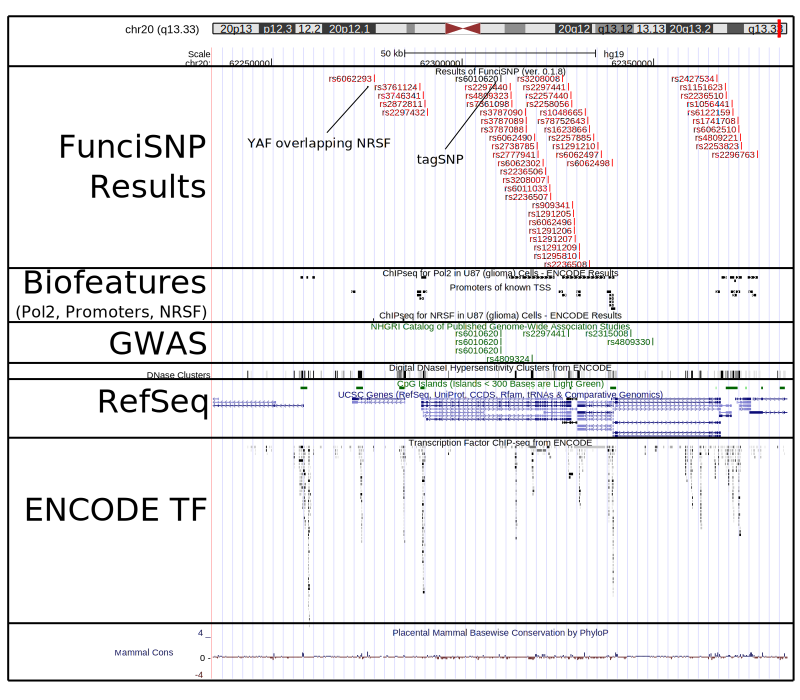
\includegraphics{UCSC_genomeviewer_glioma.pdf}                                    
\caption{\label{fig:FunciSNP_genome_viewer1.pdf} FunciSNP results viewed in UCSC
genome browser. Top track represents FunciSNP results, second track is the known
GWAS hits.}        
{\footnotesize{}}                                                                
\end{center}                                                                     
\end{figure}
%%%%%%%%%%%%%%%%%%%%%%%%%%%%%%%%%%%%%%%%%%%%%%
%%%%%%%%%%%%%%%%%%%%%%%%%%%%%%%%%%%%%%%%%%%%%%
\section{Contact information}
%%%%%%%%%%%%%%%%%%%%%%%%%%%%%%%%%%%%%%%%%%%%%%
%%%%%%%%%%%%%%%%%%%%%%%%%%%%%%%%%%%%%%%%%%%%%%
Questions or comments, please contact Simon G. Coetzee (scoetzee NEAR gmail 
 POINT com) or Houtan Noushmehr, PhD (houtana NEAR gmail POINT com).

%%%%%%%%%%%%%%%%%%%%%%%%%%%%%%%%%%%%%%%%%%%%%%
%%%%%%%%%%%%%%%%%%%%%%%%%%%%%%%%%%%%%%%%%%%%%%
\section{sessionInfo}                                                            
%%%%%%%%%%%%%%%%%%%%%%%%%%%%%%%%%%%%%%%%%%%%%%
%%%%%%%%%%%%%%%%%%%%%%%%%%%%%%%%%%%%%%%%%%%%%%

\begin{itemize}\raggedright
  \item R version 2.15.0 (2012-03-30), \verb|x86_64-pc-linux-gnu|
  \item Locale: \verb|LC_CTYPE=en_US.UTF-8|, \verb|LC_NUMERIC=C|, \verb|LC_TIME=en_US.UTF-8|, \verb|LC_COLLATE=en_US.UTF-8|, \verb|LC_MONETARY=en_US.UTF-8|, \verb|LC_MESSAGES=en_US.UTF-8|, \verb|LC_PAPER=C|, \verb|LC_NAME=C|, \verb|LC_ADDRESS=C|, \verb|LC_TELEPHONE=C|, \verb|LC_MEASUREMENT=en_US.UTF-8|, \verb|LC_IDENTIFICATION=C|
  \item Base packages: base, datasets, graphics, grDevices, grid,
    methods, splines, stats, stats4, utils
  \item Other packages: AnnotationDbi~1.18.0, Biobase~2.16.0,
    BiocGenerics~0.2.0, biomaRt~2.12.0, Biostrings~2.24.1,
    bitops~1.0-4.1, BSgenome~1.24.0,
    BSgenome.Ecoli.NCBI.20080805~1.3.17, caTools~1.12,
    ChIPpeakAnno~2.4.0, DBI~0.2-5, FunciSNP~0.1.14, gdata~2.8.2,
    GenomicFeatures~1.8.0, GenomicRanges~1.8.3, GGBase~3.18.0,
    ggplot2~0.9.0, GGtools~4.4.0, GO.db~2.7.1, gplots~2.10.1,
    gtools~2.6.2, IRanges~1.14.2, KernSmooth~2.23-7, lattice~0.20-6,
    limma~3.12.0, Matrix~1.0-6, multtest~2.12.0, org.Hs.eg.db~2.7.1,
    plyr~1.7.1, reshape~0.8.4, Rsamtools~1.8.0, RSQLite~0.11.1,
    rtracklayer~1.16.0, scales~0.2.0, snpStats~1.6.0, survival~2.36-12,
    TxDb.Hsapiens.UCSC.hg19.knownGene~2.7.1, VariantAnnotation~1.2.4
  \item Loaded via a namespace (and not attached): annotate~1.34.0,
    bit~1.1-8, colorspace~1.1-1, dichromat~1.2-4, digest~0.5.2,
    ff~2.2-6, genefilter~1.38.0, MASS~7.3-17, memoise~0.1, munsell~0.3,
    parallel~2.15.0, proto~0.3-9.2, RColorBrewer~1.0-5, RCurl~1.91-1,
    reshape2~1.2.1, stringr~0.6, tools~2.15.0, XML~3.9-4, xtable~1.7-0,
    zlibbioc~1.2.0
\end{itemize}
\textcopyleft  2012. All rights reversed (\textbf{respect the work})! This
document was proudly made using \LaTeX and \textbf{Sweave}.

hn
\end{document}
